%
% Complete documentation on the extended LaTeX markup used for Insight
% documentation is available in ``Documenting Insight'', which is part
% of the standard documentation for Insight.  It may be found online
% at:
%
%     http://www.itk.org/

\documentclass{InsightArticle}

\usepackage[dvips]{graphicx}
\usepackage{float}
\usepackage{subfigure}
\usepackage{amsmath} % for cases{}
\usepackage{graphicx}

%%%%%%%%%%%%%%%%%%%%%%%%%%%%%%%%%%%%%%%%%%%%%%%%%%%%%%%%%%%%%%%%%%
%
%  hyperref should be the last package to be loaded.
%
%%%%%%%%%%%%%%%%%%%%%%%%%%%%%%%%%%%%%%%%%%%%%%%%%%%%%%%%%%%%%%%%%%
\usepackage[dvips,
bookmarks,
bookmarksopen,
backref,
colorlinks,linkcolor={blue},citecolor={blue},urlcolor={blue},
]{hyperref}


\title{Poisson Hole Fillin in ITK and VNL}

% 
% NOTE: This is the last number of the "handle" URL that 
% The Insight Journal assigns to your paper as part of the
% submission process. Please replace the number "1338" with
% the actual handle number that you get assigned.
%
\newcommand{\IJhandlerIDnumber}{3253}

% Increment the release number whenever significant changes are made.
% The author and/or editor can define 'significant' however they like.
\release{0.00}

% At minimum, give your name and an email address.  You can include a
% snail-mail address if you like.

\author{David Doria}
\authoraddress{Rensselaer Polytechnic Institute, Troy NY}


\begin{document}

%
% Add hyperlink to the web location and license of the paper.
% The argument of this command is the handler identifier given
% by the Insight Journal to this paper.
% 
\IJhandlefooter{\IJhandlerIDnumber}


\ifpdf
\else
   %
   % Commands for including Graphics when using latex
   % 
   \DeclareGraphicsExtensions{.eps,.jpg,.gif,.tiff,.bmp,.png}
   \DeclareGraphicsRule{.jpg}{eps}{.jpg.bb}{`convert #1 eps:-}
   \DeclareGraphicsRule{.gif}{eps}{.gif.bb}{`convert #1 eps:-}
   \DeclareGraphicsRule{.tiff}{eps}{.tiff.bb}{`convert #1 eps:-}
   \DeclareGraphicsRule{.bmp}{eps}{.bmp.bb}{`convert #1 eps:-}
   \DeclareGraphicsRule{.png}{eps}{.png.bb}{`convert #1 eps:-}
\fi


\maketitle


\ifhtml
\chapter*{Front Matter\label{front}}
\fi


% The abstract should be a paragraph or two long, and describe the
% scope of the document.
\begin{abstract}
\noindent
This code provides an implementation of Poisson Hole Filling on ITK images.

\end{abstract}

\IJhandlenote{\IJhandlerIDnumber}

\tableofcontents

%%%%%%%%%%%%%%%%%
\section{Introduction}
This code provides an implementation of Poisson Hole Filling on ITK images.

This document is intended only to describe the implementation, not the theory.

%%%%%%%%%%%%%%%%%
\section{Input}

%%%%%%%%%%%%%%%%%
\section{Poisson Solver}

%%%%%%%%%%%%%%%%%
\section{Demonstration}

\begin{figure}[H]
\centering
\subfigure[Original image]{
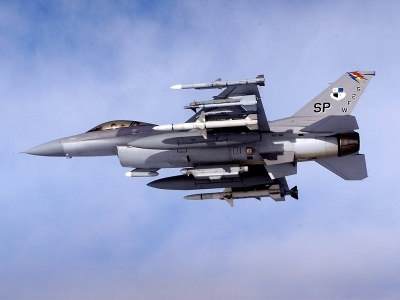
\includegraphics[width=0.3\linewidth]{images/plane}
\label{fig:Demonstration:original}
}
\subfigure[Mask]{

\includegraphics[width=0.3\linewidth]{images/planeMask}
\label{fig:Demonstration:mask}
}
\subfigure[Filled image]{

\includegraphics[width=0.3\linewidth]{images/planeFilled}
\label{fig:Demonstration:filled}
}
\caption{A demonstration of Poisson hole filling}
\label{fig:Demonstration}
\end{figure}
%%%%%%%%%%%%%%%%%
\section{Code Snippet}

Using this class is very straight forward, as shown below:

\begin{verbatim}
  PoissonEditing poissonEditing;
  poissonEditing.SetImage(imageReader->GetOutput());
  poissonEditing.SetMask(maskReader->GetOutput());
  poissonEditing.FillRegion(outputImage);
\end{verbatim}

\end{document}

